%
% nullstellen.tex -- Nullstellen von A(\omega) und Lemma von Riesz
%
% (c) 2019 Prof Dr Andreas Müller, Hochschule Rapperswil
%
\documentclass[tikz]{standalone}
\usepackage{amsmath}
\usepackage{times}
\usepackage{txfonts}
\usepackage{pgfplots}
\usepackage{csvsimple}
\usetikzlibrary{arrows,intersections,math}
\begin{document}
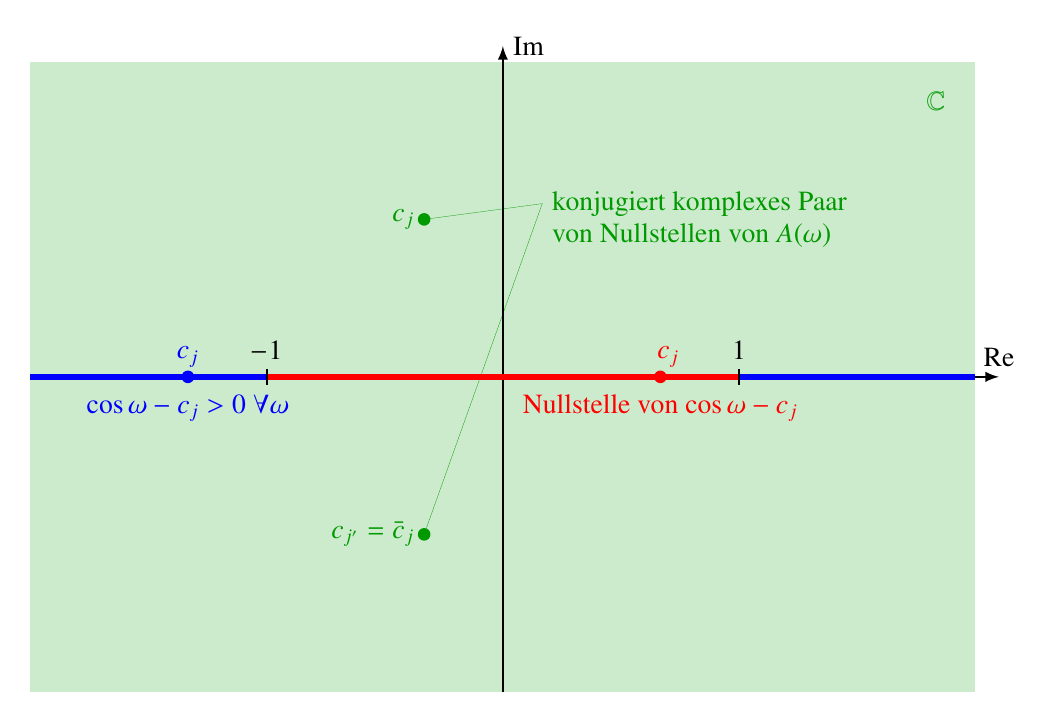
\begin{tikzpicture}[>=latex]

\definecolor{darkgreen}{rgb}{0,0.6,0}
% komplexe Ebene
\fill[color=darkgreen!20] (-6,-4) rectangle (6,4);
\node[color=darkgreen] at (5.5,3.5) {$\mathbb C$};

% Nullstellenpaar
\fill[color=darkgreen] (-1,2) circle[radius=0.08];
\fill[color=darkgreen] (-1,-2) circle[radius=0.08];
\node[color=darkgreen] at (0.5,2.2) [right] {konjugiert~komplexes Paar};
\node[color=darkgreen] at (0.5,1.8) [right] {von Nullstellen von $A(\omega)$};
\draw[line width=0.1pt,color=darkgreen] (-1,2)--(0.5,2.2);
\draw[line width=0.1pt,color=darkgreen] (-1,-2)--(0.5,2.2);
\node[color=darkgreen] at (-1,2) [left] {$c_j$};
\node[color=darkgreen] at (-1,-2) [left] {$c_{j'}=\bar{c}_j$};

% Koordinatenachsen
\draw[->,line width=0.7pt] (-6,0)--(6.3,0)
        coordinate[label={$\operatorname{Re}$}];
\draw[->,line width=0.7pt] (0,-4)--(0,4.2)
        coordinate[label={right:$\operatorname{Im}$}];

% Fall c_j \in [-1,1]
\draw[color=red,line width=2pt] (-3,0)--(3,0);

% Fall \cos\omage - c_j > 0
\draw[color=blue,line width=2pt] (3,0)--(6,0);
\draw[color=blue,line width=2pt] (-3,0)--(-6,0);
\fill[color=blue] (-4,0) circle[radius=0.08];
\node[color=blue] at (-4,0) [above] {$c_j$};
\node[color=blue] at (-4,-0.1) [below] {$\cos\omega -c_j>0\;\forall\omega$};

\node[color=red] at (2.1,0) [above] {$c_j$};
\fill[color=red] (2,0) circle[radius=0.08];
\node[color=red] at (2,-0.1) [below] {Nullstelle von $\cos\omega - c_j$};

% Ticks
\node at (3,0.1) [above] {$1$};
\draw[line width=0.7pt] (-3,-0.1)--(-3,0.1);
\node at (-3,0.1) [above] {$-1$};
\draw[line width=0.7pt] (3,-0.1)--(3,0.1);


\end{tikzpicture}
\end{document}

